% display items  -  part of main.tex (see journal/README.md)
\clearpage
\nolinenumbers

\begin{figure}[p]
\centering
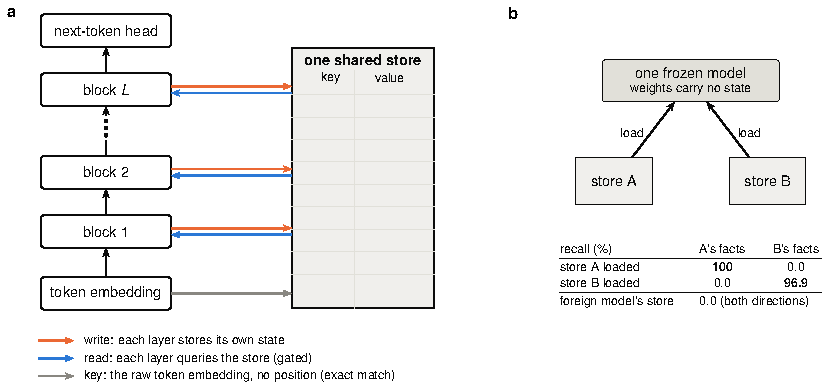
\includegraphics{fig1_architecture.pdf}
\caption{\textbf{Memory as a block.} \textbf{a}, Every layer reads from and writes its own
state into one shared store (orange arrows, writes; blue arrows, reads; grey arrow, the key). A
slot's key is the raw layer-0 token embedding without position, so retrieval is an exact token
match. Reads enter the residual stream through a gate that starts at zero, and the model keeps
no key--value cache between 128-token segments. \textbf{b}, The weights are stateless and the
store is the state. With the model frozen, loading the store that holds the queried facts gives
full recall and loading the other gives none. A store written by a differently seeded model
reads at 0\% although its facts are present, because its keys are the writer's embeddings.
$n=32$ queries per cell; 95\% intervals are in Table~1.}
\label{fig:arch}
\end{figure}

\begin{table}[p]
\centering
\small
\caption{\textbf{Core recall results.} Facts are stated once and queried out of context.
Recall is the exact match of the answer token on $n$ independent queries, with 95\% Wilson
score intervals (Methods). No hypothesis tests were used. Rows with two seeds list each
seed, and controls run at matched settings. Source data: Source Data Table~1.}
\label{tab:core}
\setlength{\tabcolsep}{4pt}
\begin{tabular}{@{}llrrl@{}}
\toprule
Experiment & Condition & $n$ & Recall (\%) & 95\% interval \\
\midrule
Facts in PG-19 prose,        & 8 facts  & 640 & 100.0 & 99.4--100.0 \\
single-token keys            & 16 facts & 640 & 100.0 & 99.4--100.0 \\
                             & 32 facts & 640 & 100.0 & 99.4--100.0 \\
                             & 64 facts & 640 & 99.1 & 98.0--99.6 \\
                             & scrambled store (64 facts) & 640 & 0.16 & 0.0--0.9 \\
\midrule
Persistence                  & store reloaded in a fresh process & 160 & 100.0 & 97.7--100.0 \\
                             & mismatched store file & 160 & 0.0 & 0.0--2.3 \\
\midrule
Placement (cold start,       & mean of all layers in one slot per token & 640 & 80.8 & 77.5--83.6 \\
32 facts)                    & each layer writes its own slot, seed 0 & 640 & 95.5 & 93.6--96.8 \\
                             & each layer writes its own slot, seed 1 & 640 & 98.9 & 97.8--99.5 \\
                             & same slots keyed by residual (control) & 640 & 0.2 & 0.0--0.9 \\
\midrule
Store as state               & store A loaded, A's facts & 32 & 100.0 & 89.3--100.0 \\
(one frozen model)           & store B loaded, B's facts & 32 & 96.9 & 84.3--99.4 \\
                             & the other store loaded (either direction) & 32 & 0.0 & 0.0--10.7 \\
                             & scrambled store & 32 & 3.1 & 0.6--15.7 \\
\midrule
Store as state               & model 1, its own store & 640 & 98.8 & 97.6--99.4 \\
(two seeded models)          & model 2, its own store & 640 & 100.0 & 99.4--100.0 \\
                             & the other model's store (either direction) & 32 & 0.0 & 0.0--10.7 \\
\bottomrule
\end{tabular}
\end{table}

\begin{figure}[p]
\centering
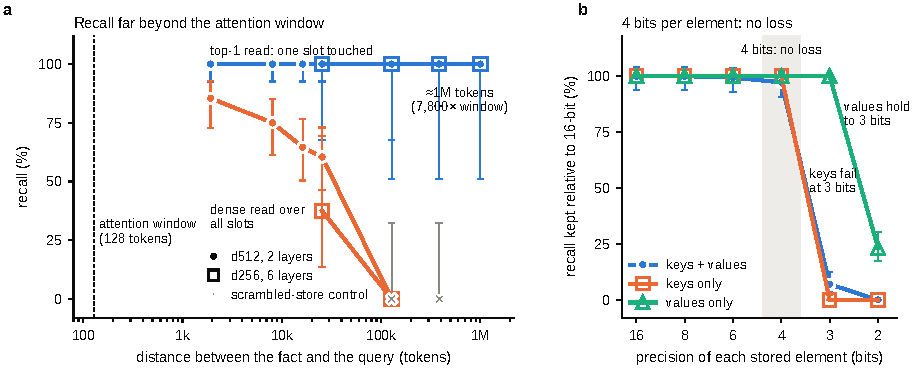
\includegraphics{fig2_longcontext.pdf}
\caption{\textbf{Recall far beyond the attention window, from a 4-bit store.}
\textbf{a}, Recall against the number of tokens between a fact and its query, for a two-layer
model (filled circles) and a six-layer model (open squares). A top-1 read, which uses one slot
(blue), stays at 100\% from 1.9k to 998k tokens, about 7,800 times the 128-token attention
window (dashed vertical line), whereas a dense read over all slots (orange) decays to 0\% by
128k tokens. Grey crosses, scrambled-store control. \textbf{b}, Recall when the stored codes are
quantized, relative to each model's unquantized recall, for keys and values together (blue
circles), keys only (orange squares) and values only (green triangles). Quantizing to 4 bits
(shaded) loses nothing and makes the store eight times smaller than at 32 bits. Keys fail at
3 bits; values hold to 3. The keys-and-values series uses a 64-fact model and the other two a
16-fact model. Error bars are 95\% Wilson intervals. In \textbf{a}, $n=48$ queries per point up
to 25k tokens and $n=4$--8 beyond (control, $n=8$), so the intervals at long range are wide; in \textbf{b}, $n=160$ per point, with the interval for the quantized recall divided by
the 16-bit recall. No hypothesis tests were used.}
\label{fig:long}
\end{figure}

\begin{figure}[p]
\centering
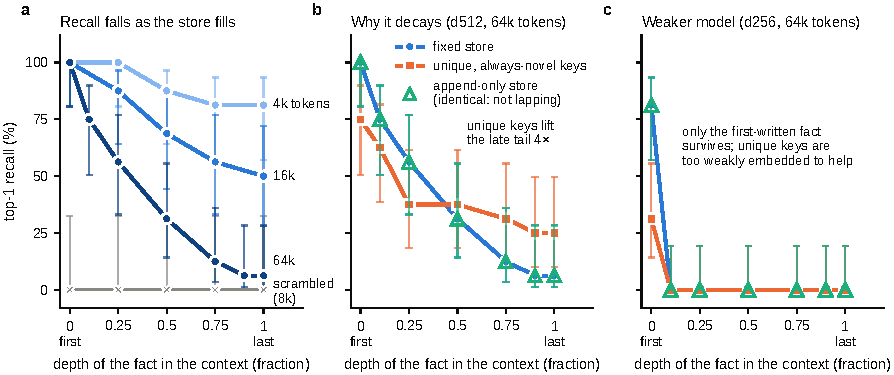
\includegraphics{fig3_passkey.pdf}
\caption{\textbf{No lost-in-the-middle, but a write-order limit.} Top-1 recall against the
depth at which the fact is written (0, first context window; 1, last before the query).
\textbf{a}, A two-layer model with 4k, 16k and 64k tokens of context (light to dark blue).
Recall falls monotonically with depth, so there is no mid-context dip, and late-written facts
are lost as the store fills. Grey crosses, scrambled store. \textbf{b}, Mechanism at 64k
tokens for the same model. An append-only store (green triangles) never overwrites and traces
a curve identical to the fixed store (blue circles). Keying facts on unique tokens, which always
pass the novelty gate (orange squares), lifts the late tail fourfold. \textbf{c}, The same for a
weaker six-layer model: only the first-written fact survives and unique keys do not help.
Panels \textbf{b} and \textbf{c} share the key. Error bars are 95\% Wilson intervals; $n=16$
queries per point (control, $n=8$). No hypothesis tests were used.}
\label{fig:passkey}
\end{figure}

\begin{figure}[p]
\centering
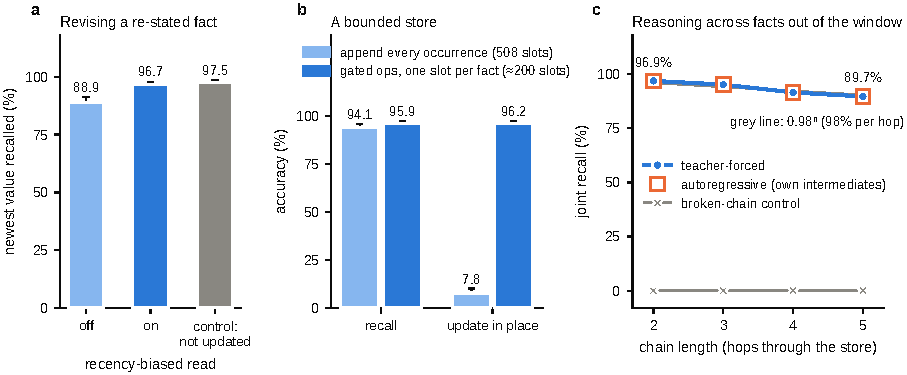
\includegraphics{fig4_memory.pdf}
\caption{\textbf{From a lookup table to a memory.} \textbf{a}, Revising a restated fact:
newest-value recall without (light blue) and with (dark blue) a recency-biased read, and for
facts that were never updated (grey). \textbf{b}, Gated write operations keep one slot per
fact: recall is maintained with about 200 slots (dark blue) instead of 508 (light blue), and
updates land in place. \textbf{c}, Multi-hop reasoning over facts held outside the context
window, by emitting each intermediate as a token and querying the store again: teacher-forced
(blue circles), autoregressive with the model's own intermediates (open orange squares) and with
one link of the chain broken (grey crosses). The grey line is 0.98 raised to the number of
hops. Two and three hops use 64 facts, four and five use 32. Error bars are 95\% Wilson
intervals; $n=640$ queries per bar or point. No hypothesis tests were used.}
\label{fig:memory}
\end{figure}
